\documentclass[12pt]{article}

\usepackage[brazilian]{babel}
\usepackage[utf8]{inputenc}
\usepackage{graphicx}
\usepackage{mathtools}
\usepackage{amsthm}
\usepackage{thmtools,thm-restate}
\usepackage{amsfonts}
\usepackage{hyperref}
\usepackage[singlelinecheck=false]{caption}
\usepackage[backend=biber,url=true,doi=true,eprint=false,style=numeric]{biblatex}
\usepackage{enumitem}
\usepackage[justification=centering]{caption}
\usepackage{indentfirst}
\usepackage{algorithm}
\usepackage{algpseudocode}
\usepackage{listings}
\usepackage[x11names,rgb,table]{xcolor}
\usepackage{tikz}
\usepackage{hyperref}
\usepackage{subcaption}
\usepackage{booktabs}
\usepackage{linegoal}
\usepackage{geometry}
\usetikzlibrary{snakes,arrows,shapes}

\addbibresource{references.bib}
\graphicspath{{imgs/}}

\makeatletter
\def\subsection{\@startsection{subsection}{3}%
  \z@{.5\linespacing\@plus.7\linespacing}{.1\linespacing}%
  {\normalfont}}
\makeatother

\makeatletter
\patchcmd{\@setauthors}{\MakeUppercase}{}{}{}
\makeatother

\DeclareMathOperator*{\argmin}{arg\,min}
\DeclareMathOperator*{\argmax}{arg\,max}
\DeclareMathOperator*{\Val}{\text{Val}}
\DeclareMathOperator*{\Ch}{\text{Ch}}
\DeclareMathOperator*{\Pa}{\text{Pa}}
\DeclareMathOperator*{\Sc}{\text{Sc}}
\newcommand{\ov}{\overline}
\newcommand{\tsup}{\textsuperscript}

\newcommand\defeq{\mathrel{\overset{\makebox[0pt]{\mbox{\normalfont\tiny\sffamily def}}}{=}}}

\newcommand{\algorithmautorefname}{Algorithm}
\algrenewcommand\algorithmicrequire{\textbf{Input}}
\algrenewcommand\algorithmicensure{\textbf{Output}}
\algnewcommand{\LineComment}[1]{\State\,\(\triangleright\) #1}

\captionsetup[table]{labelsep=space}

\theoremstyle{plain}

\newcounter{dummy-def}\numberwithin{dummy-def}{section}
\newtheorem{definition}[dummy-def]{Definition}
\newcounter{dummy-thm}\numberwithin{dummy-thm}{section}
\newtheorem{theorem}[dummy-thm]{Theorem}
\newcounter{dummy-prop}\numberwithin{dummy-prop}{section}
\newtheorem{proposition}[dummy-prop]{Proposition}
\newcounter{dummy-corollary}\numberwithin{dummy-corollary}{section}
\newtheorem{corollary}[dummy-corollary]{Corollary}
\newcounter{dummy-lemma}\numberwithin{dummy-lemma}{section}
\newtheorem{lemma}[dummy-lemma]{Lemma}
\newcounter{dummy-ex}\numberwithin{dummy-ex}{section}
\newtheorem{exercise}[dummy-ex]{Exercise}
\newcounter{dummy-eg}\numberwithin{dummy-eg}{section}
\newtheorem{example}[dummy-eg]{Example}

\numberwithin{equation}{section}

\newcommand{\set}[1]{\mathbf{#1}}
\newcommand{\pr}{\text{P}}
\newcommand{\eps}{\varepsilon}
\newcommand{\ddspn}[2]{\frac{\partial#1}{\partial#2}}
\newcommand{\iddspn}[2]{\partial#1/\partial#2}
\renewcommand{\implies}{\Rightarrow}

\newcommand{\bigo}{\mathcal{O}}

\setlength{\parskip}{1em}

\lstset{frameround=fttt,
	numbers=left,
	breaklines=true,
	keywordstyle=\bfseries,
	basicstyle=\ttfamily,
}

\newcommand{\code}[1]{\lstinline[mathescape=true]{#1}}
\newcommand{\mcode}[1]{\lstinline[mathescape]!#1!}

\newgeometry{margin=1in}
\title{%
  \vspace{-3.0cm}
  {
\includegraphics[scale=0.2]{logo-usp.png}}\\
  {\textbf{\uppercase{\Large USP --- Universidade de São Paulo}}}\\
  \vspace{1.5cm}
  {\textbf{Aprendizagem automática de redes soma-produto}}\\
  \vspace{2.0cm}
\flushleft{\Large Relatório Final de Projeto de Iniciação Científica\\
CNPq PIBIC Projeto 800585/2016\texttt{-}0}\\
  \vspace{2.5cm}
\flushleft{\Large Bolsista: Renato Lui Geh\\
Orientador: Prof.\ Dr.\ Denis Deratani Mauá}\\
  \vspace{2.5cm}
  \centering
  {\Large\textbf{São Paulo}}\\
  \vspace{0.25cm}
  {\Large\textbf{2018}}\\
}
\date{}

\begin{document}

\maketitle

\renewcommand{\abstractname}{\Large{Resumo}}

\begin{abstract}
  \vspace{0.4cm}
  \normalsize
  Modelos probabilísticos baseados em grafo (PGMs) possibilitam modelar distribuições de
  probabilidade complexas com milhares de varíaveis. Devido a grande expressividade em
  representabilidade, PGMs mostraram-se viáveis para modelagem de casos reais.

  Redes soma-produto (SPNs) são PGMs que restringem-se ao escopo de distribuições de probabilidade
  tratáveis. SPNs tiveram bons resultados em diversas aplicações, obtendo valores comparáveis a
  outros modelos estado-da-arte, porém com tempo de execução ordens de magnitude menor.

  Apesar dos resultados promissores, atualmente existem poucas bibliotecas para inferência e
  aprendizado de SPNs. Além disso, não existe atualmente uma comparação detalhada entre diferentes
  algoritmos de rede-soma produto.

  Este projeto teve dois objetivos. O primeiro foi construir uma biblioteca livre e gratuita para
  inferência e aprendizado de redes soma-produto. O segundo foi fazer uma comparação de alguns
  algoritmos de aprendizado de SPNs no domínio de classificação e compleição de imagens.\\~\\

  \textbf{Palavras-chave:} Modelos probabilísticos baseados em grafo, redes soma-produto,
  processamento de imagens
  \newpage
\end{abstract}

\section{Introdução}

Modelos probabilísticos baseados em grafos (PGM, do inglês \textit{Probabilistic Graphical Models})
representam uma distribuição de probabilidade de forma compacta. Estes modelos representados por
grafos facilitam tanto a compreensão humana ao estudá-los, quanto possibilitam que vários problemas
já existentes em Teoria dos Grafos sejam utilizados como solução para problemas em PGMs. Extrair
conhecimento de PGMs é análogo a extrair a probabilidade de um certo evento ocorrer dado que
eventos distintos tenham ocorrido. Tal extração de conhecimento é chamada de inferência. Fazer
inferência exata em PGMs clássicas, ou seja, achar a probabilidade exata de um certo evento, é
intratável. Uma solução para este problema é utilizar métodos para inferência aproximada nestes
modelos. No entanto, tais algoritmos aproximados são muitas vezes difíceis de analisar. Além disso,
como os algoritmos de aprendizado do modelo utilizam inferência como subrotina, por consequência o
aprendizado torna-se aproximado.

\begin{figure}[h]
  \centering
  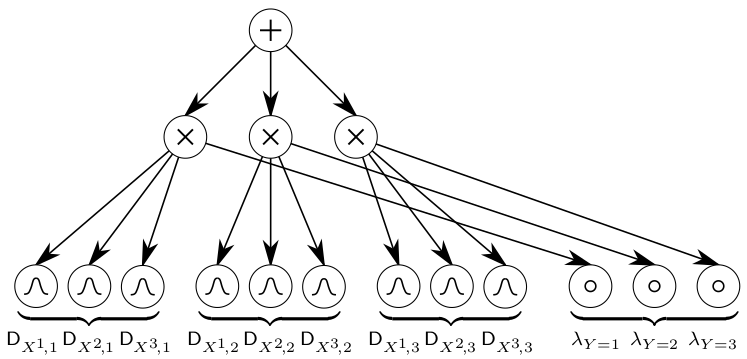
\includegraphics[scale=0.4]{nbayes.png}
  \caption{Fonte~\cite{peharz-spn}}\label{spn-example}
\end{figure}

Redes soma-produto (SPN, de \textit{Sum-Product Network}) são PGMs que representam uma distribuição
de probabilidade tratável. Proposto em 2011, SPNs computam inferência exata em tempo linear ao
número de arestas de seu grafo se sua estrutura obedecer a certas
propriedades~\cite{poon-domingos}. A~\autoref{spn-example} mostra um exemplo de rede soma-produto
representando o modelo Naïve Bayes com três atributos. SPNs apresentam uma série de características
interessantes, como sua arquitetura profunda que permite representar funções de forma mais
eficiente quanto mais profundo seu grafo~\cite{shallow-vs-deep}. Outras interessantes propriedades
teóricas incluem uma generalização de SPNs para qualquer semianel em que o produto tenha escopo
disjunto~\cite{sp-theorem}. Com relação a aplicações, SPNs tiveram resultados impressionantes em
diversas áreas, como enovelamento de proteínas~\cite{rec-dec-non-convex}, modelagem de
sinais~\cite{model-speech}, classificação e reconstrução de
imagens~\cite{gens-domingos,poon-domingos,clustering}, reconhecimento de atividade~\cite{activity}
e linguagem natural~\cite{nat-lang}.

Uma SPN pode ser definida como um DAG onde nós são somas ponderadas, produtos, variáveis
indicadoras ou distribuições de probabilidade univariadas. Uma folha de uma SPN é
sempre uma variável indicadora ou uma distribuição univariada e vice-versa. O escopo de uma SPN é o
conjunto de todas variáveis da rede. O escopo de uma folha de uma SPN é a variável descrita pela
variável indicadora ou distribuição univariada. Semânticamente, o conjunto de filhos de um nó soma
pode ser interpretado como uma relação de semelhança entre as variáveis dos escopos dos filhos,
enquanto que o conjunto de filhos de um produto pode ser visto como uma relação de independência
entre os escopos dos filhos do nó produto. O valor de um nó soma é a soma ponderada de seus filhos
em função dos pesos de suas arestas de saída. O valor de um nó produto é o produto dos valores dos
filhos e o valor de uma folha é o valor da variável indicadora ou a probabilidade da distribuição
univariada.

Apesar dos resultados expressivos, atualmente existem poucas bibliotecas para inferência e
aprendizado de redes soma-produto. Grande parte dos códigos existentes possuem pouca documentação
ou não são mais mantidos ou atualizados. Além disso, não existem comparações detalhadas entre
algoritmos de aprendizado de SPNs na literatura ou uma biblioteca que facilite esta tarefa.

Neste projeto, buscou-se criar uma biblioteca livre e gratuita para inferência e aprendizado de
redes soma-produto. Foram implementadas subrotinas para computar a probabilidade de evidência
exata, a probabilidade \textit{maximum a posteriori} aproximada de uma SPN e três métodos de
aprendizado de redes soma-produto. Adicionalmente, foram implementadas funções para auxiliar a
comparação entre diferentes arquiteturas de SPNs, verificar propriedades da estrutura da rede e
classificar e completar imagens.

\section{Objetivos}

O projeto teve como objetivos criar uma biblioteca livre e gratuita para inferência e aprendizado
de redes soma-produto e gerar dados comparativos de diversos algoritmos de aprendizado de SPNs
estado-da-arte.

Originalmente, planejava-se implementar quatro algoritmos de aprendizado. No entanto, preferiu-se
gerar um relatório mais detalhado de três algoritmos. Os três algoritmos implementados são listados
abaixo.

\begin{enumerate}[label=\alph*.]
  \item Algoritmo de Poon-Domingos~\cite{poon-domingos}
  \item Algoritmo de aprendizado estrutural de Dennis-Ventura~\cite{clustering}
  \item Algoritmo de aprendizado estrutural de Gens-Domingos~\cite{gens-domingos}
\end{enumerate}

Após as implementações, foram feitos testes de desempenho em conjuntos de dados reais e artificiais
para classificação e compleição de imagens.

\section{Metodologia}

Neste projeto, buscou-se analisar três artigos de aprendizado de redes soma-produto.

\begin{enumerate}
  \item \textit{Sum-Product Networks: A New Deep Architecture}, H. Poon e P. Domingos, UAI
    2011~\cite{poon-domingos}
  \item \textit{Learning the Structure of Sum-Product Networks}, R. Gens e P. Domingos, ICML
    2013~\cite{gens-domingos}
  \item \textit{Learning the Architecture of Sum-Product Networks Using Clustering on Variables},
    A. Dennis e D. Ventura, NIPS 2012~\cite{clustering}
\end{enumerate}

Foram implementados os algoritmos descritos e tentou-se replicar os resultados apresentados nos
artigos. Para isso, foi construída a biblioteca
GoSPN\footnote{\url{https://github.com/RenatoGeh/gospn}} na linguagem Go. A escolha da linguagem
foi dada pelo suporte nativo a programação concorrente e paralela, velocidade de execução, e por
ser uma linguagem fortemente tipada e compilada.

Após implementados os métodos de aprendizagem, foram feitos testes e comparações nos desempenhos e
acurácias dos três algoritmos nos seguintes conjuntos de dados de imagens.

\begin{enumerate}[label=\,(\alph*)]
  \item Caltech-101~\cite{caltech101}
  \item Olivetti Faces Dataset~\cite{olivetti}
  \item Digits~\cite{digits}
  \item DigitsX~\cite{digitsx}
  \item MNIST~\cite{mnist}
\end{enumerate}

\section{Resultados e Discussão}

O projeto consistiu na elaboração de três algoritmos de aprendizado. Estes algoritmos foram
implementados na biblioteca GoSPN\footnotemark[1]. Duas variações do método de otimização de
descida de gradiente foram escritas para os algoritmos de Poon-Domingos e Dennis-Ventura. Para o
algoritmo de Gens-Domingos, foram implementados dois métodos de \textit{clustering}, DBSCAN e
$k$-means. Adicionalmente, os algoritmos $k$-mode e $k$-medoid foram implementados por Diarmaid
Conaty\footnotemark[2] e Cassio P. de Campos\footnote{Queen's University Belfast} como
contribuições à biblioteca. Para os testes de independência entre variáveis foram implementados os
testes de qui-quadrado e G-test. A biblioteca também possibilita o uso de distribuições gaussianas
ou multinomiais como folhas da rede.

Para o método de otimização de descida de gradiente, foram criadas as versões \textit{soft} e
\textit{hard}. A primeira usa as derivadas parciais da SPN em função dos pesos para atualizar os
parâmetros da rede. No entanto, para o caso de redes profundas o gradiente tende a se aproximar de
zero conforme o sinal é propagado pela rede. Para evitar este problema, usa-se o segundo método.
Seja $S$ uma SPN, define-se $M$ a rede máximo-produto (MPN) de $S$ como o grafo cópia de $S$ em que
todos os nós somas são substituidos por nós máximo. O valor de um nó máximo é o maior valor
ponderado de seus filhos. O valor de uma MPN é o valor da raíz. O caminho percorrido a partir da
raíz de maior valor representa a probabilidade \textit{maximum a posteriori} (MAP). Denotaremos
por $W$ o multiconjunto de todas as arestas que pertencem ao caminho descrito pelo MAP\@. Extraindo
as derivadas da MPN $M$ e denotando $\Ch(n)$ e $\Pa(n)$ os conjuntos de filhos e pais do nó $n$
respectivamente, temos os valores descritos nas tabelas~\ref{tab:derivative-spn}
e~\ref{tab:derivative-weight}.

\begin{table}[h]
  \centering
  \begin{tabular}{l|l}
    \hline
    \multicolumn{1}{c}{\bfseries Método} & \multicolumn{1}{c}{\bfseries Derivada parcial do nó $j$}\\
    \hline & \\
    \textbf{Soft} & \(\displaystyle \ddspn{S}{S_j}=\sum_{\substack{n\in\Pa(j)\\n:\text{ soma}}}w_{n,j}\ddspn{S}{S_n}+\sum_{\substack{n\in\Pa(j)\\n:\text{ produto}}}\ddspn{S}{S_n}\prod_{k\in\Ch(n)\setminus\{j\}}S_k\) \\
    & \\
    \textbf{Hard} & \(\displaystyle
        \ddspn{M}{M_j}=\sum_{\substack{n\in\Pa(j)\\n:\text{ soma}}}
        \begin{cases}
          w_{k,n}\ddspn{M}{M_k} & \text{se $w_{k,n}\in W$}\\
          0 & \text{c.c.}
        \end{cases}
        + \sum_{\substack{n\in\Pa(j)\\n:\text{ produto}}}\ddspn{M}{M_n}\prod_{k\in\Ch(n)\setminus\{j\}}M_k
      \) \\
      & \\
    \hline
  \end{tabular}
  \caption{\label{tab:derivative-spn} As derivadas parciais da SPN em função de um nó $j$ no caso
    geral.}
\end{table}

\begin{table}[h]
  \centering
  \begin{tabular}{l|c}
    \hline
    \multicolumn{1}{c}{\bfseries Método} & \multicolumn{1}{c}{\bfseries Derivada parcial do peso}\\
    \hline & \\
    \textbf{Soft} & \(\displaystyle \ddspn{S}{w_{n,j}} = S_j\ddspn{S}{S_n} \) \\
    & \\
    \textbf{Hard} & \(\displaystyle \ddspn{M}{w_{n,j}} = M_j\ddspn{M}{M_n} \) \\
    & \\
    \hline
  \end{tabular}
  \caption{\label{tab:derivative-weight} As derivadas parciais da SPN em função da aresta $n\to j$.}
\end{table}

Todas as derivadas são em função de certa evidência. Portanto a notação $\iddspn{S}{S_j}$ equivale a
$\iddspn{S}{S_j}(X)$, onde $X$ é algum conjunto de valorações válidas para as variáveis de $S$.
Para computar o gradiente, deriva-se a log-verossimilhança da distribuição da SPN em função do
conjunto de parâmetros $w$, ou seja, $\ddspn{}{w}\log\pr(X)$, obtendo os resultados
da~\autoref{tab:gradients}.

\begin{table}[H]
  \centering
  \begin{tabular}{l|c}
    \hline
    \multicolumn{1}{c}{\bfseries Método} & \multicolumn{1}{c}{\bfseries Gradientes}\\
    \hline & \\
    \textbf{Soft} & \(\displaystyle \Delta w_{n,j} = \eta\ddspn{S}{w_{n,j}} \) \\
    & \\
    \textbf{Hard} & \(\displaystyle \Delta w_{n,j} = \eta \frac{c_{n,j}}{w_{n,j}} \) \\
    & \\
    \hline
  \end{tabular}
  \caption{\label{tab:gradients} As derivadas parciais da SPN em função da aresta $n\to j$.}
\end{table}

Onde $c_{n,j}$ denota a contagem de vezes que $w_{n,j}$ pertence a $W$. No caso do método
\textit{soft} de gradiente descendente, a atualização do peso depende da derivada parcial
$\iddspn{S}{w_{n,j}}$, enquanto que na versão \textit{hard}, $\Delta w_{n,j}$ apenas depende do
número de passagens pela aresta. É portanto possível perceber o porquê do método \textit{soft}
ter problemas com difusão de gradiente e \textit{hard} não. Testes feitos com todos os conjuntos de
dados usados mostraram que difusão de gradiente ocorreu em todos eles, o que mostra que, em
casos de mundo real é necessário o uso do método de otimização de gradiente descendente
\textit{hard}.

\begin{figure}[h]
  \begin{subfigure}{.5\textwidth}
    \centering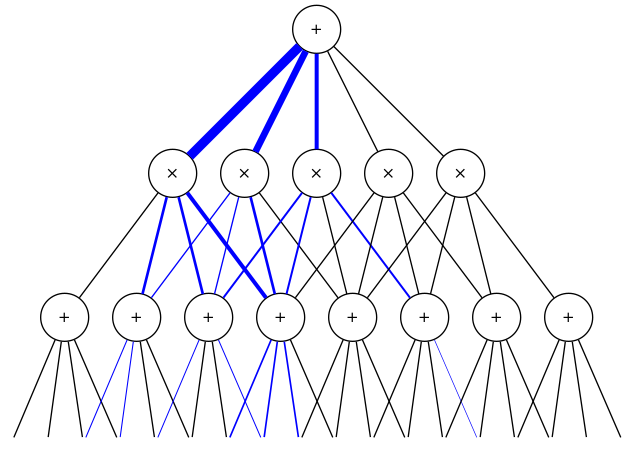
\includegraphics[scale=0.375]{graphs/softgrad.png}
    \caption{Derivação \textit{soft}}
  \end{subfigure}
  \begin{subfigure}{.5\textwidth}
    \centering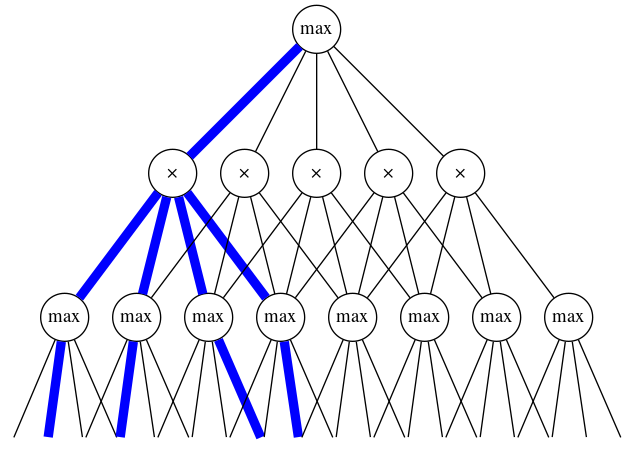
\includegraphics[scale=0.375]{graphs/hardgrad.png}
    \caption{Derivação \textit{hard}}
  \end{subfigure}
  \captionsetup{justification=raggedright}
  \caption{O gradiente no método \textit{soft} tende a se diluir conforme a altura da rede. Usando
  a derivação \textit{hard}, o gradiente não depende da derivada parcial diluída.}
\end{figure}

Para a implementação e replicação dos resultados do artigo de Poon-Domingos, foi necessário
implementar o algoritmo de geração de estrutura densa descrito no artigo. O código escrito para
este algoritmo é restrito ao domínio de imagens, no entanto, a ideia por trás da arquitetura pode
ser aplicada a qualquer domínio em que existe uma forte relação de dependência entre variáveis
locais~\cite{poon-domingos}.

A estrutura densa é formulada a partir da ideia de que existe uma relação de semelhança entre
os pixels de uma região retangular de uma imagem, e uma relação de independência entre outras
regiões retangulares que não a contém. Cada região retangular é representada por um conjunto de $m$
nós somas. Para cada região retangular, decompõe-se a região em duas partições de forma que as
partições também sejam regiões retangulares da imagem. Na SPN, representa-se esta decomposição por
um conjunto de nós produtos.

\begin{figure}[h]
  \centering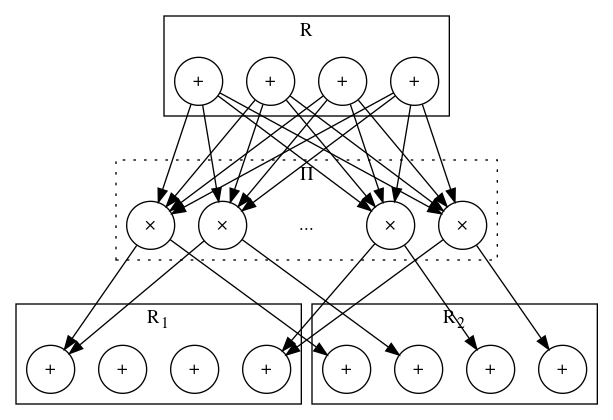
\includegraphics[scale=0.5]{graphs/decomp.png}
  \captionsetup{justification=raggedright}
  \caption{Decomposição de uma região $R$ em duas subregiões $R_1$ e $R_2$. O conjunto $\Pi$ de nós
  produtos representa a relação de independência entre as duas subregiões.}
\end{figure}

Quando $R$ representa a própria imagem, ou seja, a região retangular que engloba todos os pixels da
imagem, então o conjunto de nós somas contém apenas um nó soma. Para regiões unitárias em que a
região é apenas um pixel, ao invés de somas, geram-se $g$ gaussianas de tal forma que cada $k$
gaussiana é o $k$-ésimo quantil da distribuição dos valores do pixel. Quando a região tem dimensões
menores que $r\times r$, a chamamos de região fina. As regiões maiores ou iguais a $r\times
r$ são chamadas de regiões grosseiras. Para as regiões grosseiras tomam-se apenas partições que
geram subregiões maiores ou iguais a $r\times r$, enquanto que para regiões finas, geram-se
partições para todas as possíveis subregiões retangulares. As arestas conectando uma região $R$ ao
conjunto de produtos $\Pi$ são geradas de tal forma que todo nó soma de $R$ está conectada a todo
nó produto de $\Pi$. Porém, as arestas ligando cada produto em $\Pi$ a cada nó soma nas subregiões
$R_1$ e $R_2$ podem ou não existir. Para decidir quais arestas devem existir, escolhe-se uma
ligação $\pi_k\to\sigma_j^i$, onde $\pi\in\Pi$ e $\sigma_j^i\in R_j$, tal que esta aresta seja a
mais provável dada uma instância do conjunto de treinamento.

No código disponibilizado pelos autores do
artigo\footnote{http://spn.cs.washington.edu/spn/downloadspn.php}, o algoritmo usa \textit{hard}
Expectation-Maximization (EM) para gerar as arestas mais prováveis e decidir seus pesos, apesar do
artigo dar resultados para o método de otimização de gradiente descendente. Com o intuito de gerar
resultados mais semelhantes ao artigo possível, foi implementada a parte de se gerar as arestas
mais prováveis por \textit{hard} EM, porém a ponderação das arestas foi feita a partir do método de
gradiente.

O algoritmo de Dennis-Ventura segue uma ideia similar ao de Poon-Domingos, mantendo a relação de
localidade entre pixels. No entanto, generaliza-se a ideia de região para qualquer conjunto de
pixels similares. Para isso, usa-se métodos de \textit{clustering} para achar tais regiões.

%O primeiro contém imagens de diferentes dimensões e resoluções de 101 categorias de
%objetos. Foram escolhidas as categorias carro, motos e faces. As imagens foram padronizadas e
%redimensionadas em imagens em escala de cinza com 150 de largura e 65 de altura em resolução de
%8-bits. O \textit{dataset} está disponível em
%\url{http://www.vision.caltech.edu/Image_Datasets/Caltech101/}.

%\begin{figure}[h]
  %\centering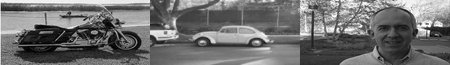
\includegraphics[scale=1.0]{imgs/caltech_sample.png}
  %\caption{Uma amostra do conjunto de dados Caltech-101.}
%\end{figure}

%O segundo é um conjunto de imagens de faces, com diferentes expressões e ângulos. As imagens têm
%dimensões $46\times 56$ com resolução de 8-bits em escala de cinza. Como a distribuição de cores é
%irregular, com nenhum pixel tendo valores extremos como a cor branca, o algoritmo de independência
%entre variáveis apresentou resultados inconsistentes. Tal problema foi resolvido diminuindo a
%resolução das imagens para 3-bits. A qualidade das imagens não sofreu grande alteração com a
%mudança. Pode-se encontrar o \textit{dataset} em
%\url{http://www.cl.cam.ac.uk/research/dtg/attarchive/facedatabase.html}.

%\begin{figure}[h]
  %\centering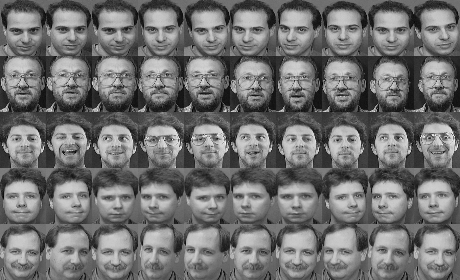
\includegraphics[scale=0.5]{imgs/olivetti_sample.png}
  %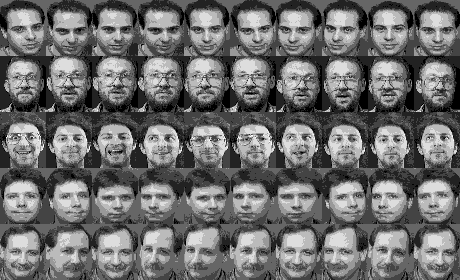
\includegraphics[scale=0.5]{imgs/olivetti-8_sample.png}
  %\captionsetup{justification=raggedright}
  %\caption{Uma amostra do conjunto de dados Olivetti. A imagem do lado esquerdo é uma amostra do
  %\textit{dataset} antes da diminuição de resolução. A imagem do lado direito mostra as imagens com
  %resolução de 3-bits.}
%\end{figure}

%O último conjunto de dados é um \textit{dataset} próprio. Foram criadas 700 imagens de dígitos de 0
%a 9, com cada dígito tendo 70 amostras. A variância das imagens em cada categoria é baixa pois o
%\textit{dataset} tem como amostra apenas a caligrafia de uma pessoa.

%\begin{figure}[h]
  %\centering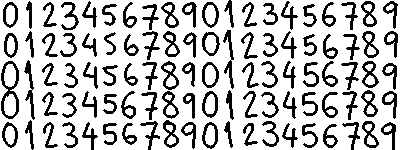
\includegraphics[scale=0.8]{imgs/digits_sample.png}
  %\caption{Uma amostra do conjunto de dados Digits.}
%\end{figure}

%Foram utilizados Caltech-101 e Digits para testes de classificação, e Olivetti para compleição de
%imagens. Para cada iteração, foi usado uma porcentagem $p$ para validação cruzada, onde $p$ é a
%porcentagem do \textit{dataset} usado para treino, e $1-p$ para teste.

%\begin{figure}[h]
  %\centering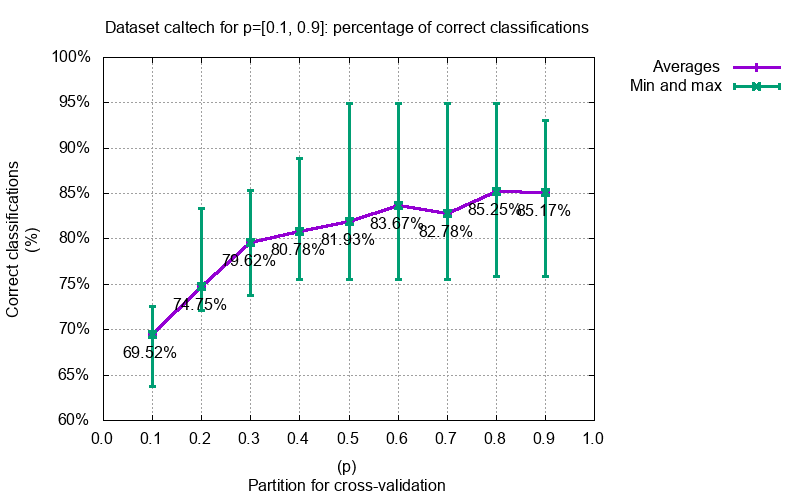
\includegraphics[scale=0.75]{imgs/caltech_percs.png}
  %\captionsetup{justification=raggedright}
  %\caption{O gráfico mostra a porcentagem de acerto no conjunto de dados Caltech-101 normalizado
  %para uma porcentagem $p$ de instâncias usadas para treino. A barra verde mostra as porcentagens
  %de acerto máximas e mínimas, enquanto que a linha azul mostra as médias das porcentagens de
  %acerto.}
%\end{figure}

%\begin{figure}[H]
  %\centering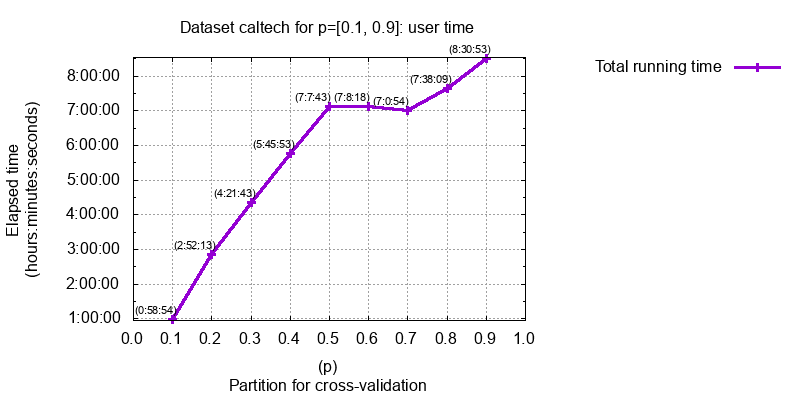
\includegraphics[scale=0.75]{imgs/caltech_time.png}
  %\captionsetup{justification=raggedright}
  %\caption{O gráfico acima mostra o tempo de aprendizado para cada $p$ no \textit{dataset}
  %Caltech-101. O tempo de inferência foi muito menor, na escala de segundos.}
%\end{figure}

%\begin{figure}[h]
  %\centering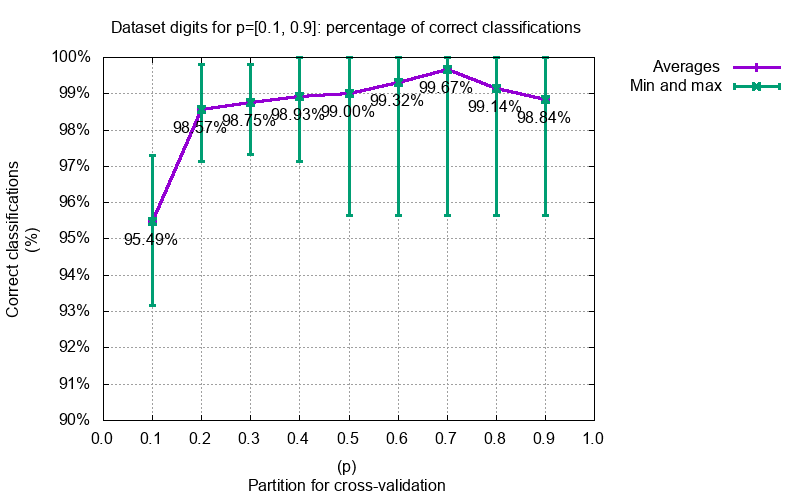
\includegraphics[scale=0.8]{imgs/digits_percs.png}
  %\caption{O gráfico mostra a porcentagem de acerto no conjunto de dados Digits.}
%\end{figure}

%\begin{figure}[H]
  %\centering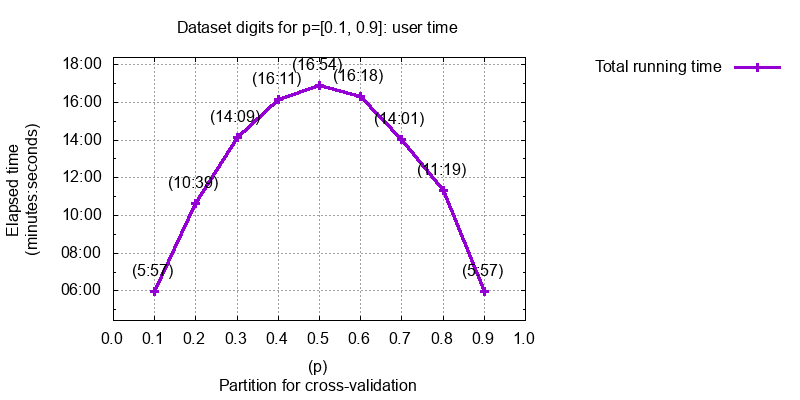
\includegraphics[scale=0.9]{imgs/digits_time.png}
  %\caption{O gráfico mostra o tempo de aprendizado para cada $p$ em Digits.}
%\end{figure}

%O conjunto Olivetti possue 10 imagens de cada pessoa em diferentes ângulos. As imagens
%diferenciam-se pela presença de acessórios, como óculos, ou por suas feições faciais, como boca
%aberta, sorriso ou olhos fechados.

%Para compleição de imagens no conjunto de dados Olivetti, foram aplicados dois testes. Em ambos
%testes foi selecionada uma imagem a ser completada, que é então removida do conjunto de treino. No
%primeiro teste, o modelo utilizou tanto as imagens de outras pessoas como as 9 imagens restantes da
%pessoa a ser completada como conjunto de treino. Chamou-se este método de teste com conhecimento
%prévio. Chamou-se de teste sem conhecimento prévio quando apenas utilizamos as faces de outras
%pessoas, descartando as 9 restantes.

%\begin{figure}[h]
  %\centering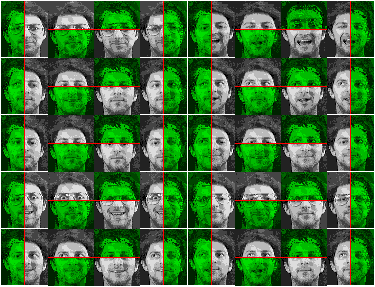
\includegraphics[scale=0.9]{imgs/c1_face_cmpl_39.png}
  %\captionsetup{justification=raggedright}
  %\caption{O resultado da compleição da parte esquerda da face dada a parte direita do rosto. Neste
  %teste houve conhecimento prévio. O modelo percebe a presença de óculos e pêlo facial.}
%\end{figure}
%\newpage

%\begin{figure}[H]
  %\centering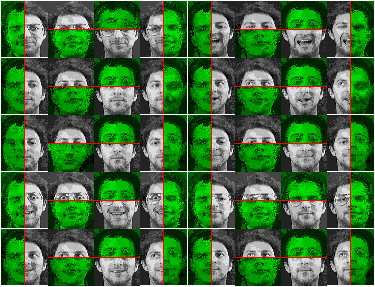
\includegraphics[scale=0.9]{imgs/c2_face_cmpl_39.png}
  %\captionsetup{justification=raggedright}
  %\caption{A mesma face, porém sem conhecimento prévio. O modelo já não percebe a presença de
  %óculos com a mesma taxa de acerto.}
%\end{figure}
\newpage

\section{Conclusão}

\printbibliography[]

\end{document}
